\documentclass{article}
\usepackage{xeCJK}
\usepackage{CJKutf8}
\setCJKmainfont{Noto Serif CJK TC}    % 思源宋體繁體版(推薦)
\setCJKsansfont{Microsoft JhengHei}   % 微軟正黑體
\setCJKmonofont{Noto Sans Mono CJK TC}
\usepackage{tikz}
\usetikzlibrary{positioning} % <--- 加這行
\tikzset{
  block/.style={rectangle, draw, rounded corners, align=center, minimum width=3cm, minimum height=1cm},
  arrow/.style={->, thick}
}

\begin{document}
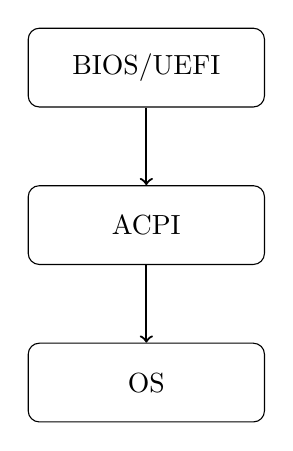
\begin{tikzpicture}[node distance=2cm]

\node[block] (bios) {BIOS/UEFI};
\node[block, below of=bios] (acpi) {ACPI};
\node[block, below of=acpi] (os) {OS};

\draw[arrow] (bios) -- (acpi);
\draw[arrow] (acpi) -- (os);

\end{tikzpicture}
\bigskip
\hrule % <-- horizontal line
\bigskip
在 Linux 開機時,許多筆電或 PC 會出現 \texttt{ACPI error / BIOS error},其原因主要包括:

\begin{itemize}
  \item \textbf{ACPI/BIOS 實作不完全符合標準}  
  ACPI 規範由 Intel 主導,但各家廠商在實作時,常為了支援特定硬體或省電機制,
  在 DSDT/SSDT(ACPI tables)中加入自訂方法。Linux kernel 解析時若遇到不符合標準的內容,就會輸出錯誤訊息。
  Windows 的 ACPI 驅動則有較強的容錯能力,因此不一定報錯。

  \item \textbf{硬體廠商針對 Windows 測試較多}  
  主流 PC/Laptop 廠商通常只針對 Windows 進行完整測試。Linux 在解析 ACPI tables 時,
  遇到僅針對 Windows 測試過的非標準方法,就可能觸發 warning 或 error。

  \item \textbf{ACPI table bug / 廠商 hack}  
  有些 BIOS/UEFI 的 ACPI tables 本身就存在 bug(如變數未定義、錯誤的 AML 指令)。
  甚至有些廠商會檢查 \texttt{OSYS} 變數(作業系統識別),若不是回報 Windows 版本,就會執行不同分支,
  可能導致 Linux 出錯。

  \item \textbf{Linux ACPI 驅動較嚴謹}  
  Linux 社群傾向將非標準或錯誤的 ACPI table 問題直接顯示出來,而不是靜默忽略,方便除錯。
  因此雖然會看到許多錯誤或警告,但系統實際上通常仍能正常工作。
\end{itemize}

\textbf{總結:}  
這些錯誤碼多半來自於 BIOS/ACPI tables 的非標準或不完整實作。
Windows 透過相容性容錯掩蓋了問題,而 Linux 則會直接記錄下來。
\end{document}
